% !TEX root = ../main.tex
% chktex-file 46
\chapter{Theoretische Grundlagen}%
\label{sec:theory}

In Kapitel~\ref{sec:related} wurde ein Überblick über das Problemumfeld der Wissensgraphkonstruktion gegeben.
Diese Arbeit baut insbesondere auf den bereits kurz vorgestellten Konzeptgraphen, Stanfords~CoreNLP Bibliothek und der PSL auf.
Für die folgenden Kapitel ist ein Grundverständnis dieser drei Themen notwendig.
Sie werden daher in den folgenden Abschnitten näher beschrieben.

\section{Wissensmodellierung mit Konzeptgraphen}%
\label{sec:theory:cg}

John F. Sowas Konzeptgraphen bilden die Basis der Graphontologie dieser Arbeit.
Wie in~\ref{sec:related:kr:history} beschrieben, sind sie ein auf Existenzgraphen basierendes logisches Kalkül.
Die vollständige Konzeptgraphsyntax geht allerdings weit über die Prädikatenlogik hinaus, da auch Modallogik und natürlichsprachliche Konzepte, wie z.~B. Fragen und Betonungen, unterstützt werden.
Da Sowas eigene Beschreibungen diesbezüglich teils etwas unklar sind, werden im folgenden lediglich die sog.~\textit{Conceptual Graphs with Cuts}~\cite{Dau2003} vorgestellt.
Sie sind eine zur Prädikatenlogik erster Ordnung äquivalente, formal spezifizierte Teilmenge der Konzeptgraphen, deren Vollständigkeit und Korrektheit bewiesen ist.

In ihrer einfachsten Form lassen sich Konzeptgraphen als ungerichtete Graphen mit drei Arten von Knoten und zwei Arten von Kanten beschreiben.
\begin{itemize}
	\item \textbf{Konzeptknoten (\textit{concepts}):}
		Entsprechen in etwa existenzquantisierten gebundenen Variablen.
		\begin{align*}
			\vcenter{\hbox{
\includegraphics[height=1.5em]{gfx/theory/conceptNode.pdf}}}
			\quad\Leftrightarrow\quad
			{\color{rot}\exists\ a, b}
		\end{align*}
	\item \textbf{Relationsknoten (\textit{conceptual relations}) und Argumentkanten (\textit{arguments}):}
		Relationsknoten entsprechen den Relationssymbolen in Atomen.
		Zwischen Relationsknoten und Konzeptknoten können Argumentkanten existieren;
		sie entsprechen den Argumenten eines prädikatenlogischen Atoms.
		Die Position der Argumente bei mehrstelligen Relationen werden durch Nummerierung der Argumentkanten oder bei zweistelligen Relationen durch gerichtete Argumentkanten abgebildet.
		\begin{align*}
			\vcenter{\hbox{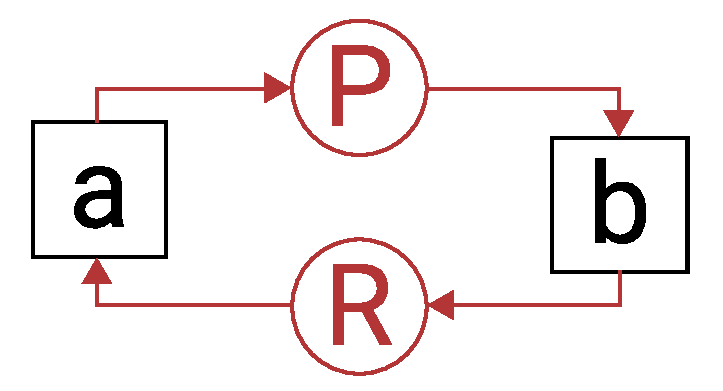
\includegraphics[height=3em]{gfx/theory/relationNode.pdf}}}
			\quad\Leftrightarrow\quad
			\exists\ a, b:\ {\color{rot}P(a, b) \land R(b, a)}
		\end{align*}
	\item \textbf{Negationskontexte (\textit{negation contexts} oder \textit{cuts}):}
		Für die Negation von Aussagen werden in Konzeptgraphen sog.~Kontexte verwendet.
		Sie lassen sich neben der Negation auch zur Modellierung anderer Zusammenhänge nutzen, diese werden hier allerdings ausgelassen, um den Vergleich mit der Prädikatenlogik zu ermöglichen.
		\begin{align*}
			\vcenter{\hbox{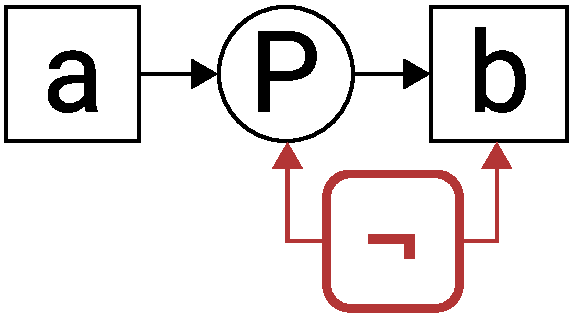
\includegraphics[height=3em]{gfx/theory/negationNode1.pdf}}}
			\quad\Leftrightarrow\quad
			\exists\ a\ {\color{rot}\lnot\exists}\ b: P(a, b)
		\end{align*}
		Die Darstellung von Kontexten mit Knoten und Kanten wird schnell unübersichtlich, daher werden stattdessen i.~d.~R. Boxen verwendet, die die Kindknoten umschließen.
		\begin{align*}
			\vcenter{\hbox{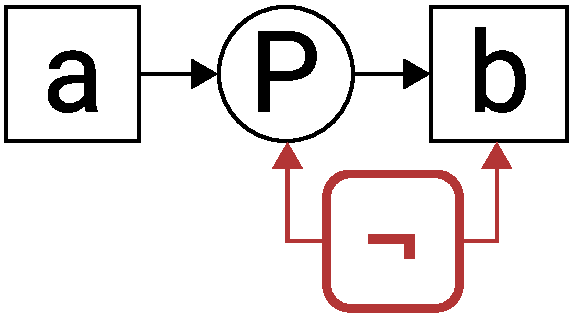
\includegraphics[height=3em]{gfx/theory/negationNode1.pdf}}}
			\quad\Leftrightarrow\quad
			\vcenter{\hbox{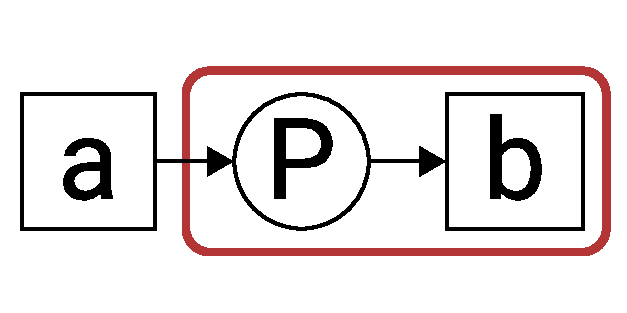
\includegraphics[height=3em]{gfx/theory/negationNode2.pdf}}}
		\end{align*}
	\item \textbf{Koreferenzkanten (\textit{coreference links}):}
		Entsprechen der Äquivalenzrelation.
\end{itemize}

\section{Stanford CoreNLP}%
\label{sec:theory:nlp}

\section{Modellierung von Hinge-Loss-MRFs mit PSL}%
\label{sec:theory:psl}
